\documentclass[12pt,english,a4paper]{article}

\usepackage[utf8]{inputenc}          % Allows UTF-8 encoded characters in the .tex-file.
\usepackage{babel,csquotes,textcomp} % Set LaTeX to structure the content following international academic standards.

\usepackage{hyperref}
\usepackage{graphicx}
\usepackage{pdfpages}
\usepackage{listings}
\usepackage{wrapfig}
\usepackage{color}
\usepackage{lettrine}
\usepackage[font={small,it}]{caption}

\usepackage[
    backend=biber,
    style=numeric
]{biblatex}
\addbibresource{refs.bib}

\definecolor{mygreen}{rgb}{0,0.6,0}
\definecolor{mygray}{rgb}{0.5,0.5,0.5}
\definecolor{mymauve}{rgb}{0.58,0,0.82}

\lstset{ %
  basicstyle=\ttfamily\small,     
  backgroundcolor=\color{white},   % choose the background color
  breaklines=true,                 % automatic line breaking only at whitespace
  captionpos=b,                    % sets the caption-position to bottom
  commentstyle=\color{mygreen},    % comment style
  escapeinside={\%*}{*)},          % if you want to add LaTeX within your code
  keywordstyle=\color{blue},       % keyword style
  stringstyle=\color{mymauve},     % string literal style
}

\title{GPS spoofing and time}
\author{Aril Johannes Schultzen}

\begin{document}

\maketitle
\thispagestyle{empty}
\setcounter{page}{0}
%\newpage
\tableofcontents
\thispagestyle{empty}
\setcounter{page}{0}
%\newpage
\thispagestyle{empty}
\setcounter{page}{0}

\begin{abstract}
Currently, this is not much more but comments and notes in order for me to write an essay, an essay meant for me to prepare for my work with my master thesis. This document does not represent the quality of the finished product in any way.
\end{abstract}

%\newpage
\clearpage
\setcounter{page}{1}

\section{Global Positioning System: A short introduction}
The Global Positioning System (GPS) is a utility owned by the United States that provides its user with positioning, navigation and timing services. At the end of 60's, the U.S Navy was developing the Polaris missile, a missile capable of being launched from a submarine. One of the requirements for launching the Polaris missile was exact knowledge of the submarines position. The problem led the Navy and The Applied Physics Laboratory at Hopkins to develop the Transit system, the earliest predecessor to the GPS system \cite{SteJ}.

Today, roughly 40 years later we are surrounded by GPS technology.
\begin{wrapfigure}{c}{0.45\textwidth}
  \centering
  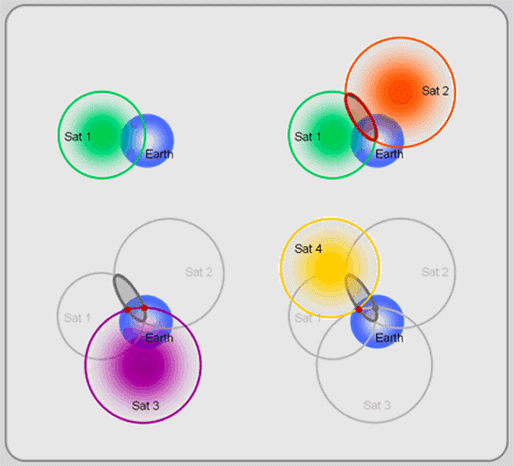
\includegraphics[width=0.40\textwidth]{trilaterate.jpg}
  \caption[GPS trilaterate figure]
   {Figure showing how GPS satellites are used to trilaterate to determine a GPS receivers position. Source: \cite{GISTRILATERATE}}
\end{wrapfigure}
In fields like emergency response, search and rescue, fleet management and even agriculture, it has become a vital tool of utmost importance to everyday operation. Satellite navigation can be found in most new cars and few phones are today sold without an internal GPS receivers. The European Space Agency estimated that there were 2 billion GPS enabled devices by 2012 \cite{ESA}. What started out as a navigation tool for the U.S navy is now used by millions, if not billions of users both civilian and military all over the globe. A common misconception (that is often reinforced by Hollywood action movies) is that the GPS satellites track \textit{you} by communicating with your GPS receiver. It actually works the other way around. You are, with your GPS receiver, tracking a set of satellites in order to establish your own position. At any given time, there are at least 24 GPS satellites each in its own orbit at about 11,000 nautical miles above your head \cite{GPSGOVSS}. In order for a GPS receiver to determine its position and obtain correct time, it will need 4 GPS satellites within line of sight \footnote{The line of sight requirement might seem unreasonable, but by the time the signal has reached earth, is has degraded to a minimum of -160 dBW \cite{NATINT}}.
The method used by your GPS receiver to determine its position is called \textit{trilateration}. 
Trilateration is used in geometry as a process of determining the location (absolute or relative) of point by measuring distance. It is often confused with triangulation which instead of distance, uses angles. Measuring the distance from the GPS satellites to a given position on earth is quite simple when using the equation: 
\begin{equation} Distance = Rate \times Time \end{equation} 
The equation is simple to solve, first we need the rate. In this context, the \textit{rate} is how fast the signals travel. This is equal to the speed of light (299,792,458 m/s). The time the signal has used traveling from the satellite to earth can be obtained by analyzing the signal itself. The signal contains a "time stamp" of when the signal was sent. By comparing this time stamp with the current time, one can calculate the age of the signal and therefore how long it has spent traveling. This is explained in greater detail under (\ref{GST}) \cite{GPSGOVTE}.  

\section{Clocks}
What does a \$10 wristwatch and a \$100 000 atomic clock have in common? They both drift. This phenomena known as \textit{clock drift}, is when a clock no longer runs at the exact same speed as a reference clock and they drift apart.
\begin{wrapfigure}{c}{0.45\textwidth}
  \centering
  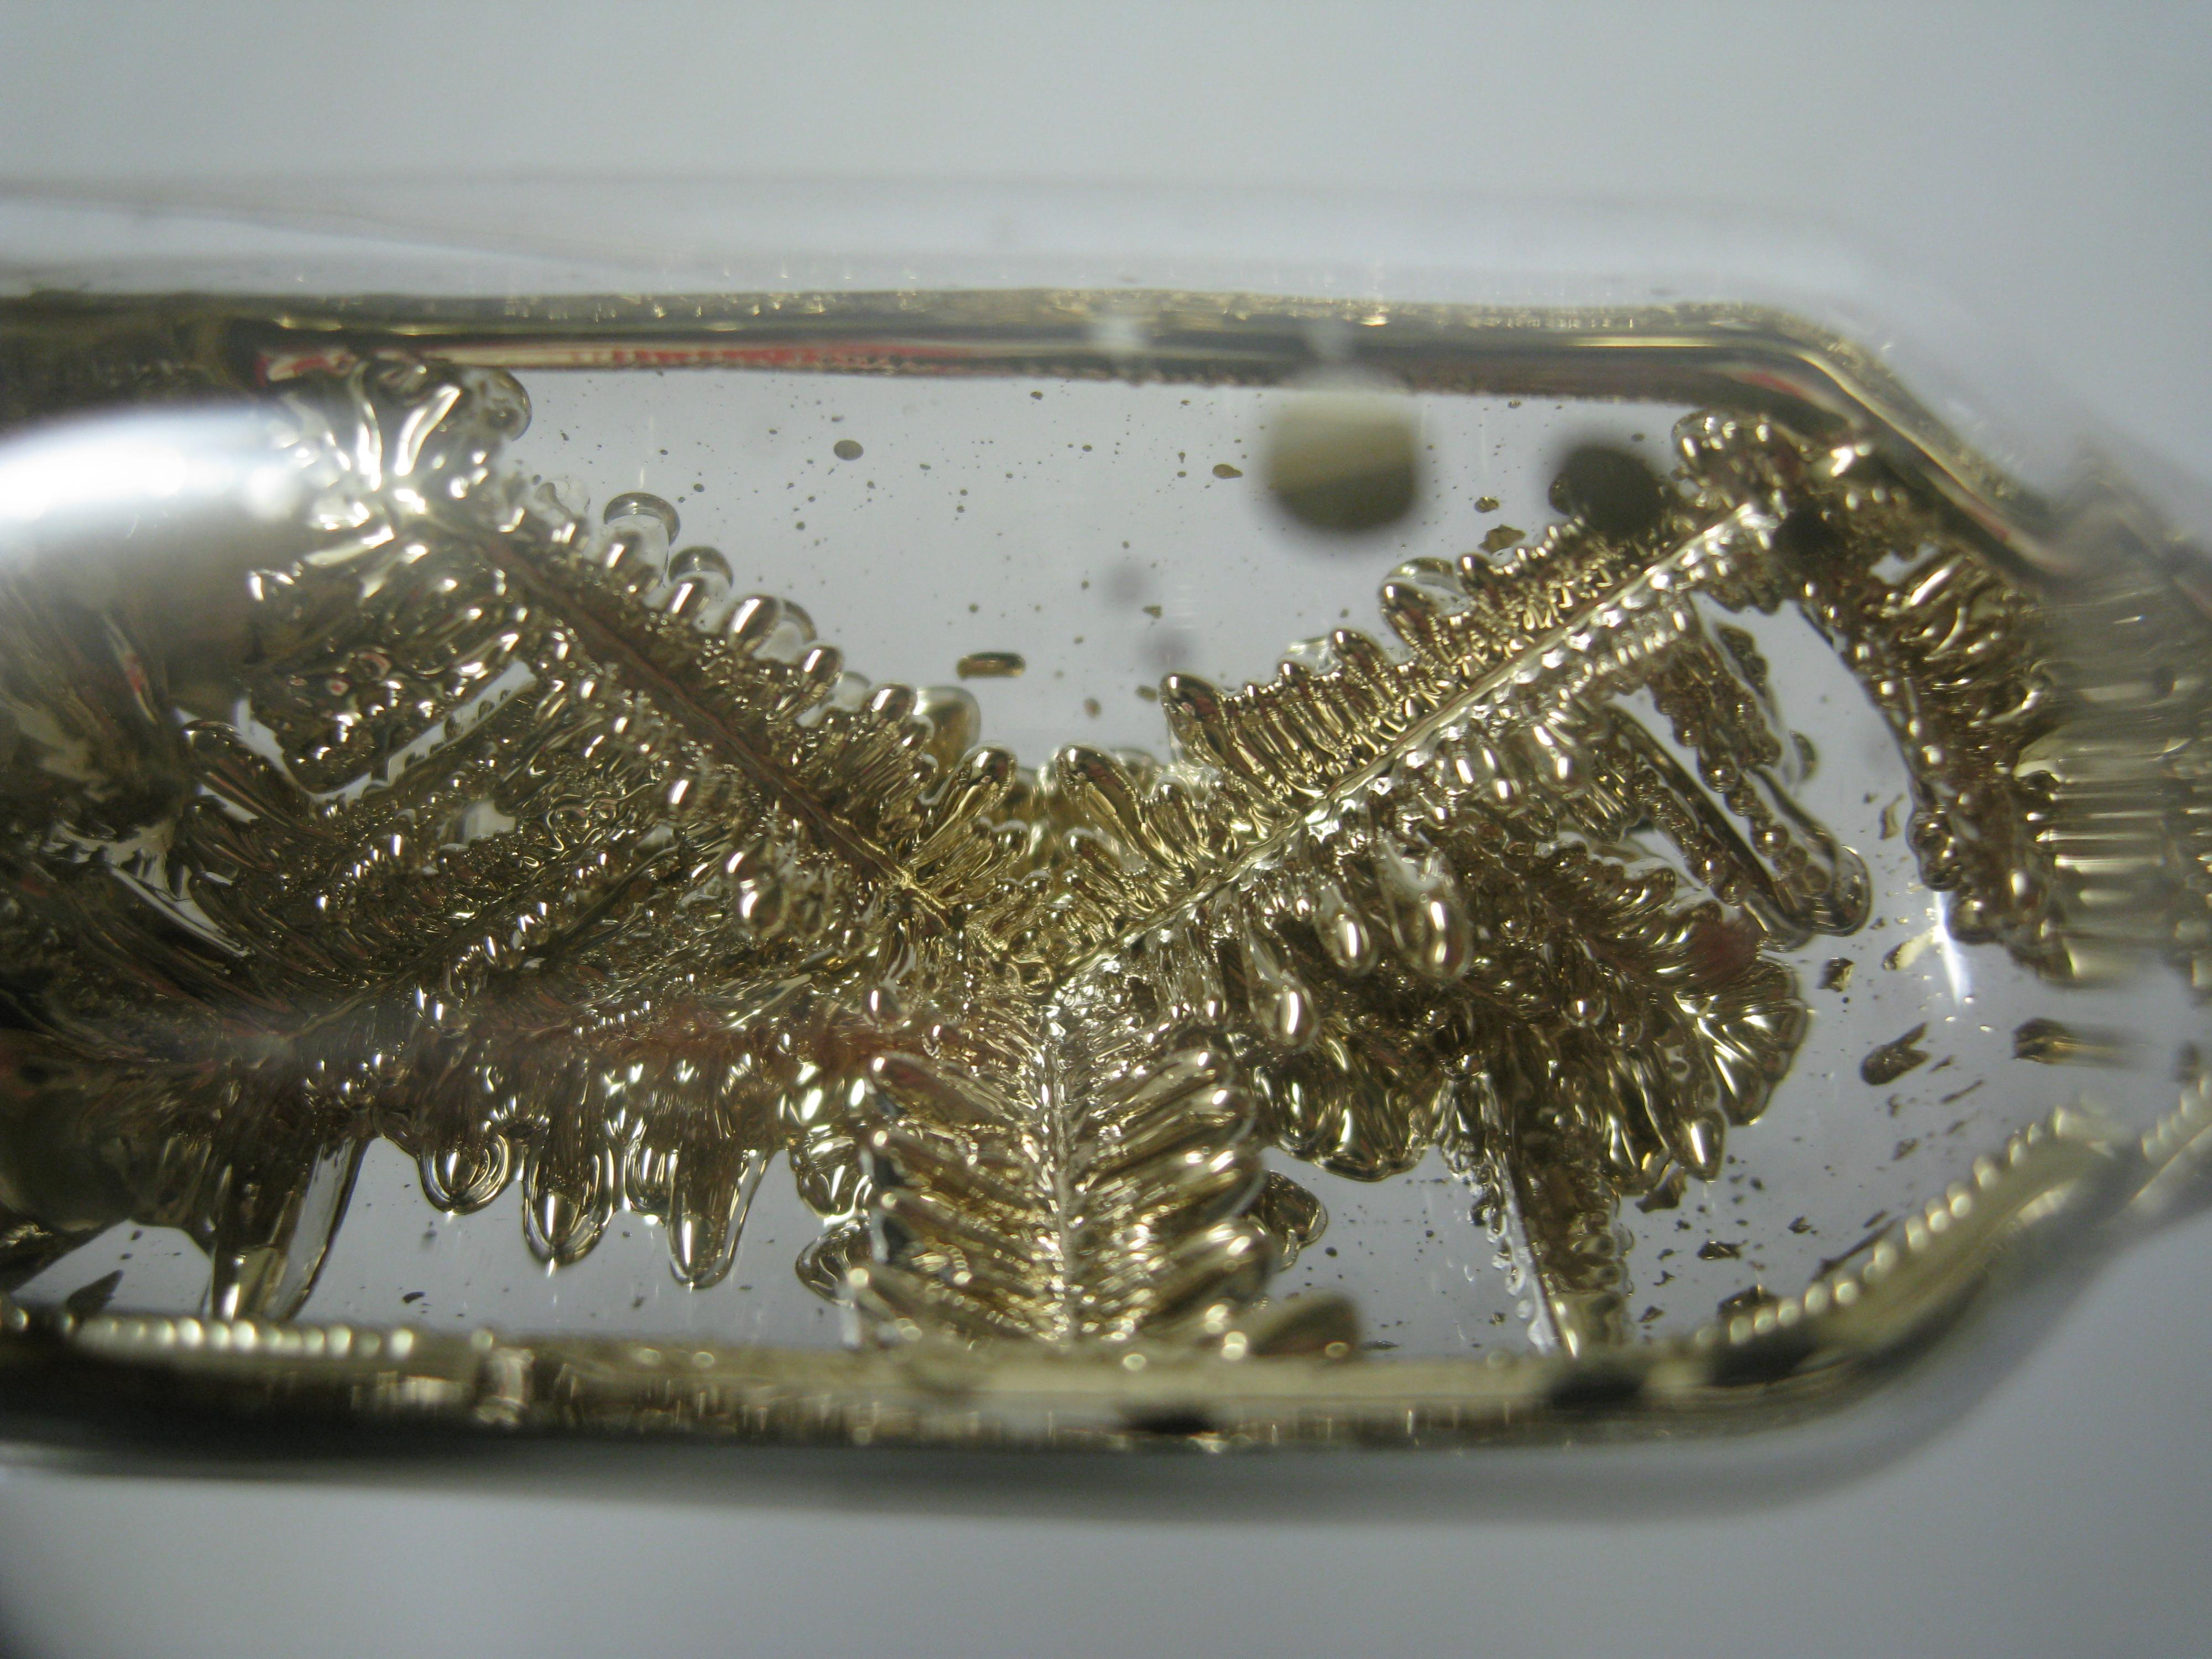
\includegraphics[width=0.40\textwidth]{cscrystals.jpg}
  \caption[Caesium campule]
   {High pure Caesium crystals in ampule under argon. Source: \cite{DENCES}}
\end{wrapfigure} 
This property is a result of how they track time. In essence, all clocks work in the same way. They have a part that oscillates, a way to count the number of oscillations and a way to show the count. If we transfer this analogy to the typical "grandfather clock", the pendulum would be the oscillator, the counting mechanism the clockwork and the clock face and dials would be the display. In a typical wristwatch, the oscillator is a quartz crystal powered by a battery. The frequency of which the crystal oscillates is then divided down to a single Hertz by simple electronics. The purity of the crystal is among the decisive factors determining the accuracy of the clock. \cite{CSMG}. 
Although a completely different beast, the same principles apply to the atomic clock which uses the microwave radiation that electrons in atoms emit when they change energy levels. One of the most commonly used elements in atomic clocks, is \textit{caesium-133}, an isotope of caesium.\footnote{1 second equals 9,192, 631,770 cycles of the Cs-133 transition} \cite{HP}. Bear in mind that this is of course an extremely limited explanation.

\section{GPS signals and Time}\label{GST}
During the introduction of this essay the properties of GPS as a tool for navigation was made apparent. This is however not the only use of GPS, it is also used for timing. The GPS satellites transmits a \textit{Coarse/Acquisition (C/A)} code and a restricted \textit{Precision (P)} code. The C/A code is freely open for everyone and is transmitted at the L1 carrier frequency (1575.42 MHz) and the P code is transmitted at both L1 and L2 (1227.60 MHz), P is reserved for the military. The C/A code is a 1023 bit pseudo random code that is transmitted at 1.023 Mbit/s, which means it repeats itself every millisecond. Each satellite transmits a different pseudo random code, codes that does not correlate well with each other. This is important because it makes it possible to separate the satellites from each other. The way the receiver calculates the distance from itself to the satellites is by comparing the pseudo random code received from the satellite with an identical one it generates itself. The receiver "slides" these codes over each other further and further until they match up. The signals travel time is determined by how far the codes have to be slided. This is what is called \textit{Code-phase GPS} and it has got some problems. Since the code have a wide cycle width, almost a microsecond, there is a lot of slop and at the speed of light, a microsecond is roughly 300 meters. What many receivers do is that they start with the code-phase and moves on to using measurements based on the carrier frequency. Since the frequency is much higher, the slop decreases and the accuracy increases dramatically. This is whats known as \textit{Carrier-phase GPS}. 

\section{Phasor Measurement Units}
An example of an application relying on GPS derived time is a PMU (phasor measurement unit).A PMU analyzes the waves on the electrical grid and uses a common time source for synchronization. This synchronization allows for real-time measurements between multiple points in the grid by multiple PMU's. The common time source (and why PMU's are relevant) is often obtained by using GPS. \cite{YLJRNR} The value of such a device is understood clearer by recognizing that the power grid is a complex, interconnected, interdependent network. In other words, errors and abnormalities in one part of the grid will have an effect on operation elsewhere and in some cases lead to whole spread blackouts \cite{EVPMUGA}.

\section{Threat Models and countermeasures}
The thread models and countermeasures presented is based on the article \textit{Reliable GPS-Based Timing for Power Systems: A Multi-Layered, Multi Receiver} by L. Heng, D. Chou and G. Xingxin Gao (2012). 
\subsection{Threats}
\subsubsection{Jamming}\label{jam}
By emitting a high-power signal at the frequencies used by GPS satellites, one can interfere with the signals received by the GPS receiver, effectively denying GPS receivers use of these signals. These signals are already weak considering their travel from space. Such an "attack", although effective, is pretty naive and easily recognized by the jammed party. If your equipment is operational and you don't have a signal, you are probably being jammed.

\subsubsection{Signal-level Spoofing}\label{sls}
Signal-level spoofing is when an attacker causes an receiver to loose lock on an authentic GPS signal by overpowering it with a false signal. This can be achieved by using a GPS simulator that matches the authentic signals phase, code delay and encoded data \cite{SGRCOOPMU}. Knowing the signal that the victim is receiving is important in order to successfully spoof it. To anyone with access to the military-grade GPS signals, this is less of an issue (tough still possible) since their signals are encrypted and harder to spoof, the civilian frequencies on the other hand are publicly known and readily predictable. Shepard, Humphreys and Fansler (2012)\cite{EVPMUGA} describes in their paper \textit{Evaluation of the Vulnerability of Phasor Measurement Units to GPS Spoofing Attacks}, a way to successfully spoof a GPS signal used by a PMU.They describe how they "introduce" the counterfeit signal to the victim by adjusting the power of the signal below the victim receivers noise floor and then gradually raises it until it surpasses the authentic signals strength. Once the victims receiver locks on, the attacker has gained full control.

\subsubsection{Data-level Spoofing}\label{dls}
In data-level spoofing, the contents (data) of the GPS signal are manipulated. GPS signals includes a variety of signal, among them the ephemeris data used to solve the positions of each satellite in orbit and also the time and status of the satellite constellation. By altering this data the receiver solves incorrect velocity, location and most important in this context, clock offset.\cite{SGRCOOPMU}

\subsubsection{Replay spoofing}\label{rs}
Replay spoofing (or \textit{meaconing}\footnote{\textit{Meacon} is portmanteau of \textit{Masking Beacon}}) is a technique where GPS signals are intercepted and rebroadcasted. The rebroadcast can be delayed and used to confuse navigation or to cause delay in applications relying on GPS signals for time.

\subsubsection{Malfunctions}\label{mf}
Just like any tool or device, a GPS receiver is prone to failure. This threat may not be posed by an external party, but is still a threat to normal operation. The ability to differentiate between an attack and a malfunction is important when deciding a response in such an event.

\subsection{Countermeasures}
\subsubsection{Monitoring Signal Power} %[C1]
In any kind of attack, jamming or spoofing, a counterfeit signal must overpower the authentic signal in order for the receiver to lock onto it or in the case with jamming, denying the authentic signal. By monitoring the strength of the signal and detecting a spike or rise in signal power, a possible attack can be identified. This is a low-cost, low-complexity and independent (in contrast to for example using other receivers as a reference) countermeasure. It is however because of the unpredictable nature of signals, not considered to be a detection confident countermeasure and should therefore only be used along side other countermeasures.\cite{HengChouGao14}

\subsubsection{Checking solved position against known position} %[C7]
By checking the position solution against the known position of the receiver, both receiver errors (\ref{mf}) and a replay spoofing (\ref{dls}) attack can be detected. It does however fall short when more sophisticated techniques like Data and Signal-level spoofing (\ref{dls},\ref{sls}) are used. These kind of attacks when done properly (unless it's done with intention), will not alter the solved position. It is important to note that this only relevant when only using \textit{one} receiver. If the position solution from multiple receivers deployed in the same area are cross-checked, this countermeasure can still be considered effective. Consider the following scenarios when using 3 receivers:
\begin{itemize}
  \item \textbf{None of the receivers are spoofed:} Each receivers solved position matches their respective known position. They all solve the same time. 
  \item \textbf{One or two receivers are spoofed:} The spoofed receiver(s) solve(s) different time compared to the receiver(s) not being spoofed.
  \item \textbf{All the receivers are spoofed:} As long as they are spoofed by the same spoofer, they will solve the same time but also the same position which again makes it possible to detect the attack.
\end{itemize}
A possible way to for a attacker to avoid detection would be to use one spoofer per receiver. These spoofers would need to be synchronized and their signal power fine tuned to make sure that they only spoof their respective receiver. It is believed that such an attack would be to complex and costly to be considered practical. \cite{HengChouGao14}

\subsubsection{Checking time solutions against receiver clock statistics} %[C8]
By comparing statistics create by monitoring the receivers clock with the time solution, one can detect spoofing (\ref{sls},\ref{dls}) as well as malfunctions (\ref{mf}). This is because the time solution is unlikely to be consistent with the statistics in event of an attack. Since this countermeasure relies on the receivers clock which can be described as both unpredictable and stochastic, it should only be used along side other countermeasures.\cite{HengChouGao14}    


\subsubsection{Cross-checking navigation data among receivers} %[C5]
When under a data-level spoofing attack (\ref{dls}), the navigation data is modified. By comparing one GPS receivers navigation data with another, both data-level spoofing and malfunctions (\ref{mf}) can be detected. This countermeasure can also prove useful during jamming attacks (\ref{jam}) because a jammed receiver could use the data from other receivers in the event that is unable to correctly decode navigation, but still able to track satellites. This may enable the receiver to continue operation during an attack. \cite{HengChouGao14}  

\subsubsection{Comparing navigation data and reverse-calculated satellite positions} %[C6]
The PMU GPS receivers are never moved and their position is known. By using their pseudorange measurements, the satellites positions can be reverse calculated by using trilateration. Since the reverse-calculated positions only match the positions calculated from the navigation data when both pseudorange and navigation data is correct, one can effectively detect replay spoofing (\ref{rs}) and malfunctions (\ref{mf}). Its also worth noting that this countermeasure increases the difficulty of both signal and data-level spoofing (\ref{dls},\ref{sls}) because it narrows down the possible valid (seemingly) spoofing signals. \cite{HengChouGao14} 

\subsubsection{Cross-correlating P(Y) code} %[C2]
This countermeasure assumes two receivers with at least 1 km distance from each other that tracks a signal from a satellite visible to them both. It is also based on the assumption that the encrypted military P(Y) code cannot be forged by a spoofer. The receivers can use the C/A code phase and timing relationships to the P(Y) code to obtain two samples from the same time frame of the received P(Y) code and then correlate the two samples. Even though the samples will be encrypted, noisy and perhaps distorted by narrow-band RF front-end, a high correlation peak should be created when a cross-correlation is conducted as long as the receivers are not spoofed. A key conclusion of the research made by L. Heng (2013) as referenced by L. Heng \textit{et alia} (2014) was that the probability of detection errors using this method decreased exponentially with the length of the samples made from the P(Y) code and the number of receivers used as reference. This method has therefore proved itself effective against spoofing attacks (\ref{dls},\ref{sls}), but ineffective against replay spoofing because the rebroadcast uses authentic GPS signals with correct P(Y) code. It is important to note that the implementation of this countermeasure relies on the GPS receivers ability to output baseband samples and that these samples are able to transfer over data network. Because the sampling rate of the samples are fairly high, it is recommended that the spoofing detection is done periodically instead of continuously. \cite{HengChouGao14}  


\newpage
\printbibliography[title={Complete Bibliography},heading=bibintoc]

\end{document}                    